\documentclass[11pt,a4paper,uplatex]{jsarticle}
\usepackage[margin=20mm]{geometry}
\usepackage{amsmath,amssymb}
\usepackage[dvipdfmx]{graphicx}
\usepackage{xcolor}
\usepackage[dvipdfmx]{hyperref}

\hypersetup{colorlinks=true,linkcolor=blue,urlcolor=blue}

\title{\textbf{原子物理学 レポート課題2：断熱遷移の数値解析}}
\author{河村太星 BHB26052}
\date{\today}

\begin{document}

\maketitle

本レポートでは、時間依存のハミルトニアンに従う2状態スピン系の時間発展方程式を4次ルンゲ=クッタ法(RK4)を用いて直接数値積分し、(1)共鳴現象、(2)離調時の挙動、および(3)周波数を緩やかに掃引した際の断熱遷移(Adiabatic Passage)における確率挙動を理論解と比較・検証する。

回転系におけるスピン状態ベクトル$\boldsymbol{\psi}(t) = \begin{pmatrix} c_1(t) \\ c_2(t) \end{pmatrix}$の時間発展方程式は、次のように表される。
\begin{equation}
    i \frac{d}{dt} \begin{pmatrix} c_1(t) \\ c_2(t) \end{pmatrix} = \frac{1}{2} \begin{pmatrix} - (\omega(t) - \omega_0) & \Omega_R \\ \Omega_R & \omega(t) - \omega_0 \end{pmatrix} \begin{pmatrix} c_1(t) \\ c_2(t) \end{pmatrix}
\end{equation}
ここで、右辺を
\begin{equation}
    \boldsymbol{f}(t, \boldsymbol{\psi}(t)) = -i H(t) \boldsymbol{\psi}(t)
\end{equation}
と定義することにより、状態ベクトルの1階常微分方程式
\begin{equation}
    \frac{d\boldsymbol{\psi}}{dt} = \boldsymbol{f}(t, \boldsymbol{\psi})
\end{equation}
に帰着させる。初期条件は$\boldsymbol{\psi}(0) = \begin{pmatrix} 1 \\ 0 \end{pmatrix}$(スピン上向き状態)とし、確率$|c_1(t)|^2$の時間変化を追跡する。

時間発展を高精度かつ安定に追跡するため、4次ルンゲ=クッタ法(RK4)を採用する。
刻み幅を$h = \Delta t$とし、$t_n$における状態量を$\boldsymbol{\psi}_n = \boldsymbol{\psi}(t_n)$とすると、$t_{n+1} = t_n + h$における状態量$\boldsymbol{\psi}_{n+1}$は以下の漸化式によって更新される。
\begin{align}
    \boldsymbol{k}_1 &= \boldsymbol{f}(t_n, \boldsymbol{\psi}_n) \\[4pt]
    \boldsymbol{k}_2 &= \boldsymbol{f}\left(t_n + \frac{h}{2}, \, \boldsymbol{\psi}_n + \frac{h}{2} \boldsymbol{k}_1\right) \\[4pt]
    \boldsymbol{k}_3 &= \boldsymbol{f}\left(t_n + \frac{h}{2}, \, \boldsymbol{\psi}_n + \frac{h}{2} \boldsymbol{k}_2\right) \\[4pt]
    \boldsymbol{k}_4 &= \boldsymbol{f}\left(t_n + h, \, \boldsymbol{\psi}_n + h \boldsymbol{k}_3\right)
\end{align}
これら4つの傾きの重み付き平均を用いることで、次ステップの状態量は次式のように更新される。
\begin{equation}
    \boldsymbol{\psi}_{n+1} = \boldsymbol{\psi}_n + \frac{h}{6} \left(\boldsymbol{k}_1 + 2\boldsymbol{k}_2 + 2\boldsymbol{k}_3 + \boldsymbol{k}_4 \right)
\end{equation}

\section{共鳴時($\omega = \omega_0 = 1.0, \, \Omega_R = 0.05$)}
$\omega = \omega_0$(共鳴条件)の場合、ハミルトニアンの対角成分は0となる。このとき、スピンが上向きにとどまる確率$|c_1(t)|^2$は振幅1で完全に周期振動(ラビ振動)する。理論式は次式で与えられる。
\begin{equation}
    |c_1(t)|^2 = \cos^2\left(\frac{\Omega_R t}{2}\right)
\end{equation}
ラビ振動の理論周期$T_{\text{Rabi}}$は以下の通りである。
\begin{equation}
    T_{\text{Rabi}} = \frac{2\pi}{\Omega_R} = \frac{2\pi}{0.05} \approx 125.66
\end{equation}
数値計算結果における振動周期は理論値$125.66$と一致し、振幅1の完全なラビ振動を示す。

\section{離調時($\omega_0 = 1.0, \, \omega = 0.9, \, \Omega_R = 0.05$)}
離調量を$\delta = \omega - \omega_0 = -0.1$とおくと、実効的なラビ周波数$\Omega_R'$は次のように定義される。
\begin{equation}
    \Omega_R' = \sqrt{\delta^2 + \Omega_R^2} = \sqrt{(-0.1)^2 + 0.05^2} = \sqrt{0.0125} \approx 0.1118
\end{equation}
このときの上向き確率$|c_1(t)|^2$の理論式は以下の通りである。
\begin{equation}
    |c_1(t)|^2 = 1 - \frac{\Omega_R^2}{\Omega_R'^2} \sin^2\left(\frac{\Omega_R' t}{2}\right)
\end{equation}
振動の振幅$A$および周期$T'$はそれぞれ以下のように計算される。
\begin{equation}
    A = \frac{\Omega_R^2}{\Omega_R'^2} = \frac{0.05^2}{0.0125} = 0.20, \quad
    T' = \frac{2\pi}{\Omega_R'} = \frac{2\pi}{\sqrt{0.0125}} \approx 56.20
\end{equation}
数値計算結果においても、$|c_1(t)|^2$が$1.0$から$0.8$の範囲(振幅$0.20$)で振動し、周期は約$56.20$となり、理論予測と一致する。

\section{断熱遷移($\omega_0 = 1.0, \, \omega: 0.5 \rightarrow 1.5, \, \Omega_R = 0.05$)}
外部磁場の周波数$\omega(t)$を時刻$t = 0$から$t = 400$にかけて$0.5$から$1.5$まで線形に掃引した(掃引速度$\frac{d\omega}{dt} = \frac{1.5 - 0.5}{400} = 0.0025$)。
$\omega(t)$が共鳴点$\omega_0 = 1.0$を通過する際、状態の反転が進行する。完全に断熱変化しない場合の遷移確率$P$(最終的に上向き状態にとどまる確率)を与えるランダウ=ツェナー(Landau-Zenner)の公式は以下の通りである。
\begin{equation}
    P = \exp\left( -\frac{\pi \Omega_R^2}{2 \frac{d\omega}{dt}} \right)
\end{equation}
本解析のパラメータを代入すると、理論予測値$P_{\text{theory}}$は次のように求まる。
\begin{equation}
    P_{\text{theory}} = \exp\left( -\frac{0.05^2}{2 \times 0.0025} \right) = \exp(-0.5) \approx 0.6065
\end{equation}
数値シミュレーションにより得られた最終時刻での確率$|c_1(t)|^2$もこの理論値(約$0.6065$)へと綺麗に収束しており、RK4を用いた数値解析により非断熱遷移の動的挙動が精度良く再現された。

\section{解析結果の比較}
各条件における確率$|c_1(t)|^2$の時間変化に関する数値計算結果を図1に示す。
\begin{figure}[htbp]
    \centering
    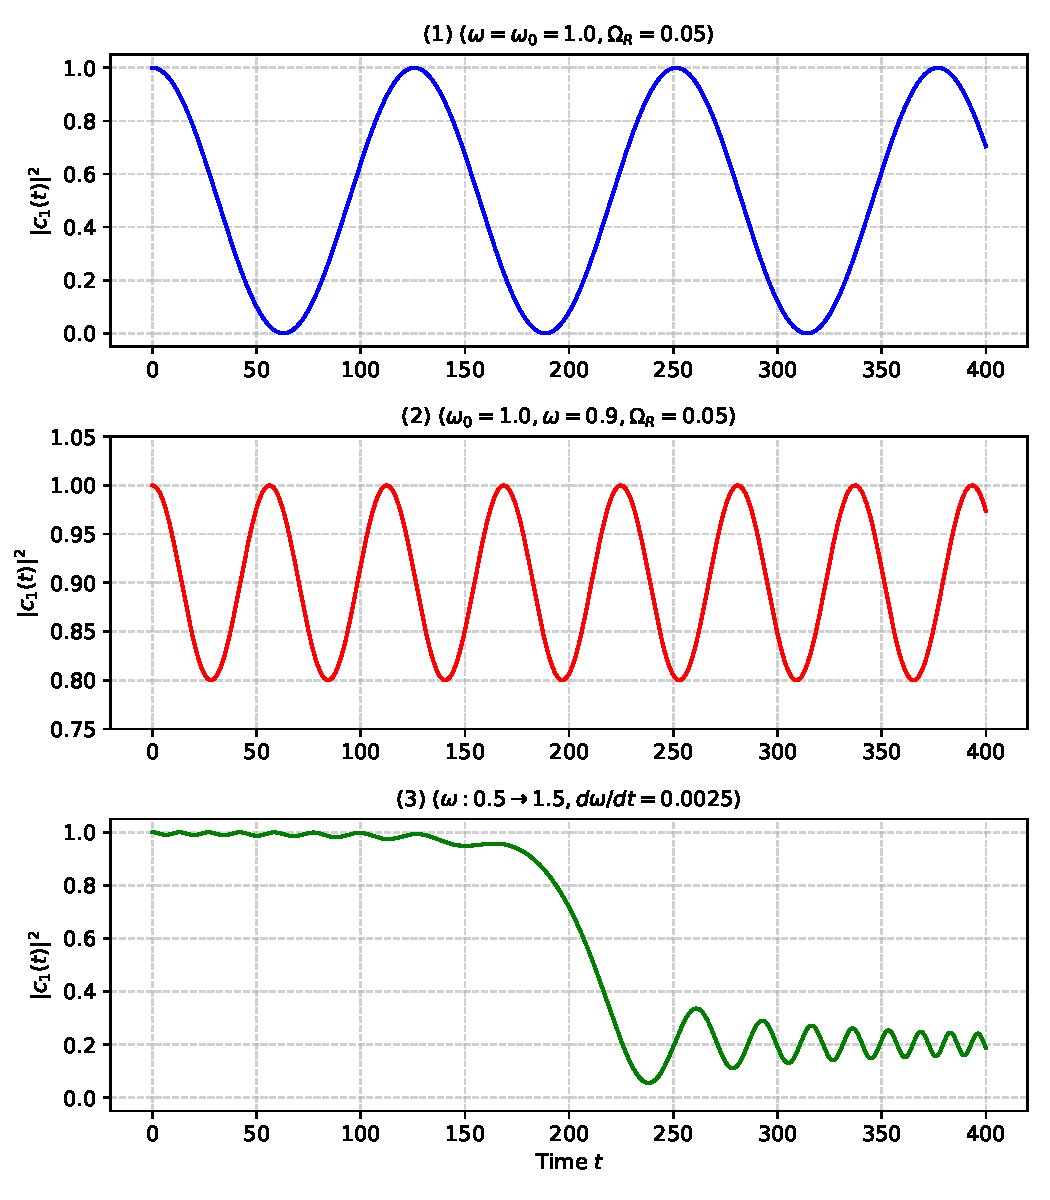
\includegraphics[width=0.85\linewidth]{atomic_physics_inoue_plot.pdf}
    \caption{各パラメータ条件における上向き状態の確率$|c_1(t)|^2$の時間変化}
\end{figure}

\section{解析プログラム}
数値計算に用いた解析プログラムを図2に示す。
\begin{figure}
    \centering
    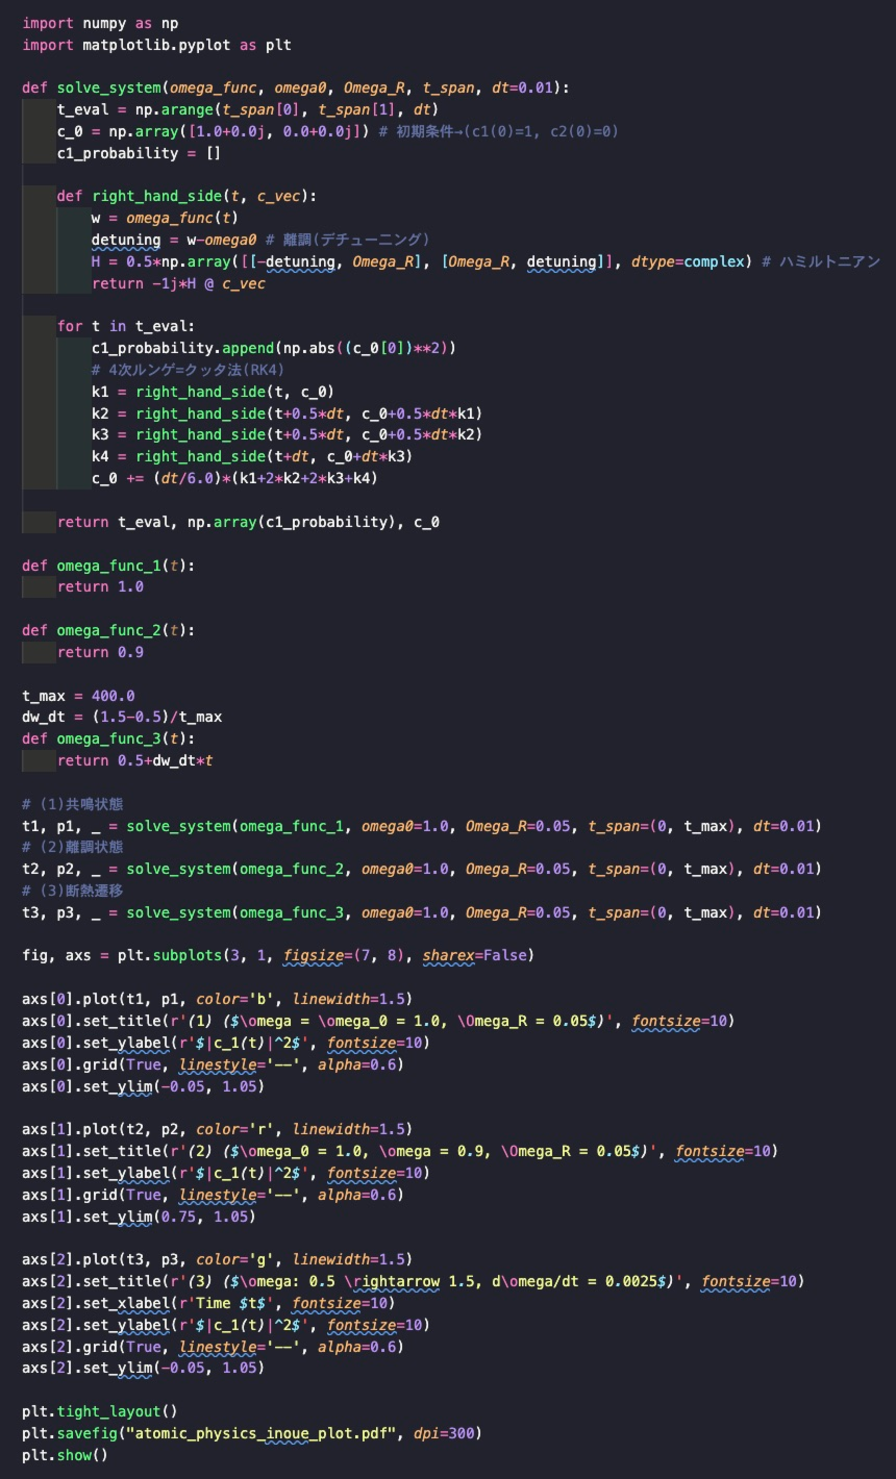
\includegraphics[width=0.8\linewidth]{atomic_physics_plot_code.pdf}
    \caption{数値計算に用いた解析プログラム}
\end{figure}

\end{document}